\documentclass{beamer}

\usepackage[utf8]{inputenc}
\usepackage[slovene]{babel}
\usepackage{default}
\usepackage{graphicx}
\usepackage{amsmath}
\usepackage{overpic}

\newcommand{\odvod}[2]{\frac{\partial #1}{\partial #2}}
\renewcommand{\vec}{\mathbf}
\newcommand{\eps}{\varepsilon}
\newcommand{\E}{\vec E}
\newcommand{\B}{\vec B}
\newcommand{\angl}[1]{(\textit{angl. #1})}

\begin{document}
\title{Modeliranje \v sirjenja svetlobe vzdol\v z ograjenih teko\v cekristalnih defektnih linij}
\author{\begin{tabular}{rl}Avtor & Miha \v Can\v cula \\ Mentor & prof. dr. Slobodan \v Zumer \\ Somentor & doc. dr. Miha Ravnik\end{tabular}}
\date{3. september 2013}

\begin{frame}
 \titlepage
\end{frame}

\begin{frame}{Teko"ci kristali}
 \begin{columns}[t]
  \column{.5\textwidth}
  
  \begin{block}{Teko"ci kristali}
   \begin{itemize}
    \item Lastnosti teko"cin in kristalov
    \item Orientacijski red
      \begin{itemize}
	\item Direktor $\vec n$
	\item Stopnja reda $S$
	\item Simetrija $\vec n \leftrightarrow -\vec n$
      \end{itemize}
      
    \item Delni pozicijski red
   \end{itemize}
  \end{block}
  
  \begin{block}{Opti"cne lastnosti}
   \begin{itemize}
    \item Dvolomnost
    \item Nadzor z zunanjimi polji
   \end{itemize}
  \end{block}

  \column[T]{.5\textwidth}
    \includegraphics[width=\textwidth]{./Slike/tvorjenje2}
    
  \end{columns}
\end{frame}

\begin{frame}{Elektromagnetno valovanje}

\begin{block}{Maxwellove ena"cbe}
\begin{equation*}
\begin{aligned}
 \nabla \cdot \vec D = \rho_f & \qquad \nabla \cdot \vec B = 0 \\
 \nabla \times \vec E = -\odvod{\vec B}{t} & \qquad \nabla \times \vec H = \vec J_f + \odvod{\vec D}{t}
\end{aligned} 
\end{equation*}
\end{block}

\begin{block}{Konstitutivni zvezi}
\begin{equation*}
\begin{aligned}
\vec D = \boldsymbol\varepsilon \varepsilon_0 \vec E \qquad \vec B = \boldsymbol \mu \mu_0 \vec H
\end{aligned} 
\end{equation*}
\end{block}

\begin{itemize}
 \item $\boldsymbol\eps$ in $\boldsymbol\mu$ sta anizotropna tenzorja
 \item Ohmov zakon $\vec J = \sigma \vec E$
 \item V vzorcu ni prostih nabojev ($\rho_f = 0$)
\end{itemize}

\end{frame}

\begin{frame}{Defekti}
 \includegraphics[width=.25\textwidth]{g_defect_2}
 \includegraphics[width=.25\textwidth]{g_defect_-2}
 \includegraphics[width=.25\textwidth]{g_defect_1}
 \includegraphics[width=.25\textwidth]{g_defect_-1}

 \begin{itemize}
  \item Obmo"cje zmanj"sanega reda
  \item Ovojno "stevilo -- celo za vektorska polja, polcelo za direktor
 \end{itemize}
 
\end{frame}


\begin{frame}{Numeri"cna metoda}
 \begin{block}{Metoda kon"cnih diferenc v "casovni domeni -- FDTD}
  \begin{itemize}
   \item "Casovni razvoj vseh 6 komponent $\vec E$ in $\vec B$
   \item Dinami"cni Maxwellovi ena"cbi na diskretni mre"zi
   \begin{equation*}
     \odvod{\vec{B}}{t} = -\nabla \times \vec{E} \qquad \odvod{\vec{E}}{t} = \eps^{-1} (\nabla \times \vec{B} - \sigma \vec E)
   \end{equation*}
    \item Komponente polj znane na razli"cnih krajih ob razli"cnih "casih
    \item Izvor in absorpcija valovanja na robu
  \end{itemize}
 \end{block}
\end{frame}

\begin{frame}{Primeri uporabe metode}
\begin{columns}[c]

\begin{column}[T]{.5\textwidth}
\begin{itemize}
 \item "Sirjenje po praznem prostoru
 \includegraphics[width=.9\textwidth]{./Slike/empty}
 
 \item Lom pri Brewsterjevem kotu
 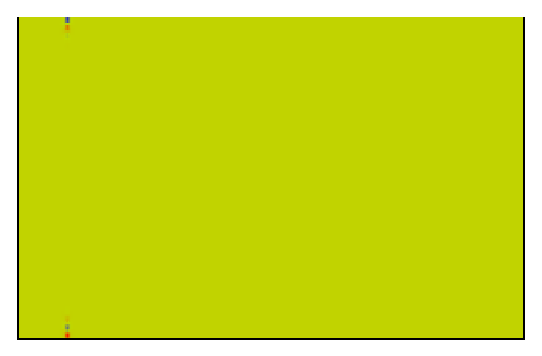
\includegraphics[width=.9\textwidth]{./Slike/refraction}

 \item Fotonski kristal

\end{itemize}

\end{column}

\begin{column}[T]{.5\textwidth}
\begin{itemize}
  \item Uniformen dvolomni kristal \\
  \hspace{-.5cm}\resizebox{.9\textwidth}{!}{\input{g_test_uniform}}
  
 \item Dvolomno vlakno
  \includegraphics[width=.41\textwidth]{./Slike/licp_0_68} \hspace{2pt}
  \includegraphics[width=.41\textwidth]{./Slike/licp_0_78}
\end{itemize}

\end{column}

\end{columns}

\end{frame}


\end{document}
